%% abtex2-modelo-trabalho-academico.tex, v-1.9.7 laurocesar
%% Copyright 2012-2018 by abnTeX2 group at http://www.abntex.net.br/ 
%%
%% This work may be distributed and/or modified under the
%% conditions of the LaTeX Project Public License, either version 1.3
%% of this license or (at your option) any later version.
%% The latest version of this license is in
%%   http://www.latex-project.org/lppl.txt
%% and version 1.3 or later is part of all distributions of LaTeX
%% version 2005/12/01 or later.
%%
%% This work has the LPPL maintenance status `maintained'.
%% 
%% The Current Maintainer of this work is the abnTeX2 team, led
%% by Lauro César Araujo. Further information are available on 
%% http://www.abntex.net.br/
%%
%% This work consists of the files abntex2-modelo-trabalho-academico.tex,
%% abntex2-modelo-include-comandos and abntex2-modelo-references.bib
%%
% ------------------------------------------------------------------------
% ------------------------------------------------------------------------
% abnTeX2: Modelo de Trabalho Academico (tese de doutorado, dissertacao de
% mestrado e trabalhos monograficos em geral) em conformidade com 
% ABNT NBR 14724:2011: Informacao e documentacao - Trabalhos academicos -
% Apresentacao
% ------------------------------------------------------------------------
% ------------------------------------------------------------------------
%%
%% Documento ajustado para PCS-EPUSP em 15/mar/2023 por Cintia Borges Margi
% ------------------------------------------------------------------------
%%
\documentclass[
	% -- opções da classe memoir --
	12pt,				% tamanho da fonte
	openright,			% capítulos começam em pág ímpar (insere página vazia caso preciso)
	oneside,			% para impressão em recto e verso. Oposto a oneside
	a4paper,			% tamanho do papel. 
	% -- opções da classe abntex2 --
	%chapter=TITLE,		% títulos de capítulos convertidos em letras maiúsculas
	%section=TITLE,		% títulos de seções convertidos em letras maiúsculas
	%subsection=TITLE,	% títulos de subseções convertidos em letras maiúsculas
	%subsubsection=TITLE,% títulos de subsubseções convertidos em letras maiúsculas
	% -- opções do pacote babel --
	english,			% idioma adicional para hifenização
	french,				% idioma adicional para hifenização
	spanish,			% idioma adicional para hifenização
	brazil				% o último idioma é o principal do documento
	]{abntex2}

% ---
% Pacotes básicos 
% ---
\usepackage{lmodern}			% Usa a fonte Latin Modern			
\usepackage[T1]{fontenc}		% Selecao de codigos de fonte.
\usepackage[utf8]{inputenc}		% Codificacao do documento (conversão automática dos acentos)
\usepackage{indentfirst}		% Indenta o primeiro parágrafo de cada seção.
\usepackage{color}				% Controle das cores
\usepackage{graphicx}			% Inclusão de gráficos
\usepackage{microtype} 			% para melhorias de justificação
% ---
		
% ---
% Pacotes adicionais, usados apenas no âmbito do Modelo Canônico do abnteX2
% ---
\usepackage{lipsum}				% para geração de dummy text
% ---
\usepackage{longtable}
\usepackage{tikz}
\usepackage{amsmath}
\usepackage{float}

% Definição de cores para prioridades
\definecolor{alta}{RGB}{200,0,0}
\definecolor{media}{RGB}{200,120,0}
\definecolor{baixa}{RGB}{0,140,0}
 
\newcommand{\palta}{\textcolor{alta}{\textbf{Alta}}}
\newcommand{\pmedia}{\textcolor{media}{\textbf{Média}}}
\newcommand{\pbaixa}{\textcolor{baixa}{\textbf{Baixa}}}


% ---
% Pacotes de citações
% ---
\usepackage[brazilian,hyperpageref]{backref}	 % Paginas com as citações na bibl
\usepackage[alf]{abntex2cite}	% Citações padrão ABNT

%% CBM: pacote para incluir a ficha catalográfica como pdf
\usepackage[final]{pdfpages}

% --- 
% CONFIGURAÇÕES DE PACOTES
% --- 

% ---
% Configurações do pacote backref
% Usado sem a opção hyperpageref de backref
\renewcommand{\backrefpagesname}{Citado na(s) página(s):~}
% Texto padrão antes do número das páginas
\renewcommand{\backref}{}
% Define os textos da citação
\renewcommand*{\backrefalt}[4]{
	\ifcase #1 %
		Nenhuma citação no texto.%
	\or
		Citado na página #2.%
	\else
		Citado #1 vezes nas páginas #2.%
	\fi}%
% ---

% ---
% Informações de dados para CAPA e FOLHA DE ROSTO
% ---
\titulo{Especificação do TCC: Aplicando medidas de segurança na transferência de dados em conectores OBD-II}
\autor{Davi Félix de Lima, Rodrigo Sales Marcolin, Rodrigo Sinato Fernandes}
\local{São Paulo, SP}
\data{2026}
\orientador{Prof. Dr. Victor Takashi Hayashi}
\coorientador{}
\instituicao{%
  Universidade de São Paulo -- USP
  \par
  Escola Politécnica
  \par
  Departamento de Engenharia de Computação e Sistemas Digitais (PCS)}
\tipotrabalho{Monografia de Conclusão de curso (Graduação)}
% O preambulo deve conter o tipo do trabalho, o objetivo, 
% o nome da instituição e a área de concentração 
% \preambulo{Trabalho de conclusão de curso apresentado ao Departamento de Engenharia de Computação e Sistemas Digitais da Escola Politécnica da Universidade de São Paulo para obtenção do Título de Engenheiro.}
% ---


% ---
% Configurações de aparência do PDF final

% alterando o aspecto da cor azul
\definecolor{blue}{RGB}{41,5,195}

% informações do PDF
\makeatletter
\hypersetup{
     	%pagebackref=true,
		pdftitle={\@title}, 
		pdfauthor={\@author},
    	pdfsubject={\imprimirpreambulo},
	    pdfcreator={LaTeX with abnTeX2},
		pdfkeywords={abnt}{latex}{abntex}{abntex2}{trabalho acadêmico}, 
		colorlinks=true,       		% false: boxed links; true: colored links
    	linkcolor=blue,          	% color of internal links
    	citecolor=blue,        		% color of links to bibliography
    	filecolor=magenta,      		% color of file links
		urlcolor=blue,
		bookmarksdepth=4
}
\makeatother
% --- 

% ---
% Posiciona figuras e tabelas no topo da página quando adicionadas sozinhas
% em um página em branco. Ver https://github.com/abntex/abntex2/issues/170
\makeatletter
\setlength{\@fptop}{5pt} % Set distance from top of page to first float
\makeatother
% ---

% ---
% Possibilita criação de Quadros e Lista de quadros.
% Ver https://github.com/abntex/abntex2/issues/176
%
\newcommand{\quadroname}{Quadro}
\newcommand{\listofquadrosname}{Lista de quadros}

\newfloat{quadro}{loq}{\quadroname}[chapter]
\newlistof{listofquadros}{loq}{\listofquadrosname}
\newlistentry{quadro}{loq}{0}

% configurações para atender às regras da ABNT
\setfloatadjustment{quadro}{\centering}
\counterwithout{quadro}{chapter}
\renewcommand{\cftquadroname}{\quadroname\space} 
\renewcommand*{\cftquadroaftersnum}{\hfill--\hfill}

\setfloatlocations{quadro}{hbtp} % Ver https://github.com/abntex/abntex2/issues/176
% ---

% --- 
% Espaçamentos entre linhas e parágrafos 
% --- 

% O tamanho do parágrafo é dado por:
\setlength{\parindent}{1.3cm}

% Controle do espaçamento entre um parágrafo e outro:
\setlength{\parskip}{0.2cm}  % tente também \onelineskip

% ---
% compila o indice
% ---
\makeindex
% ---

% ----
% Início do documento
% ----
\begin{document}

% Seleciona o idioma do documento (conforme pacotes do babel)
%\selectlanguage{english}
\selectlanguage{brazil}

% Retira espaço extra obsoleto entre as frases.
\frenchspacing 

% ----------------------------------------------------------
% ELEMENTOS PRÉ-TEXTUAIS
% ----------------------------------------------------------
% \pretextual

% ---
% Capa
% ---
% \imprimircapa
% ---

% ---
% Folha de rosto
% (o * indica que haverá a ficha bibliográfica)
% ---
\imprimirfolhaderosto*
% ---

% ---
% Inserir a ficha bibliografica
% ---

% Isto é um exemplo de Ficha Catalográfica, ou ``Dados internacionais de
% catalogação-na-publicação''. Você pode utilizar este modelo como referência. 
% Porém, provavelmente a biblioteca da sua universidade lhe fornecerá um PDF
% com a ficha catalográfica definitiva após a defesa do trabalho. Quando estiver
% com o documento, salve-o como PDF no diretório do seu projeto e substitua todo
% o conteúdo de implementação deste arquivo pelo comando abaixo:
%
%% TODO: utilizar a ficha catalográfica gerada em https://www.poli.usp.br/bibliotecas/servicos/catalogacao-na-publicacao
% \begin{fichacatalografica}
%     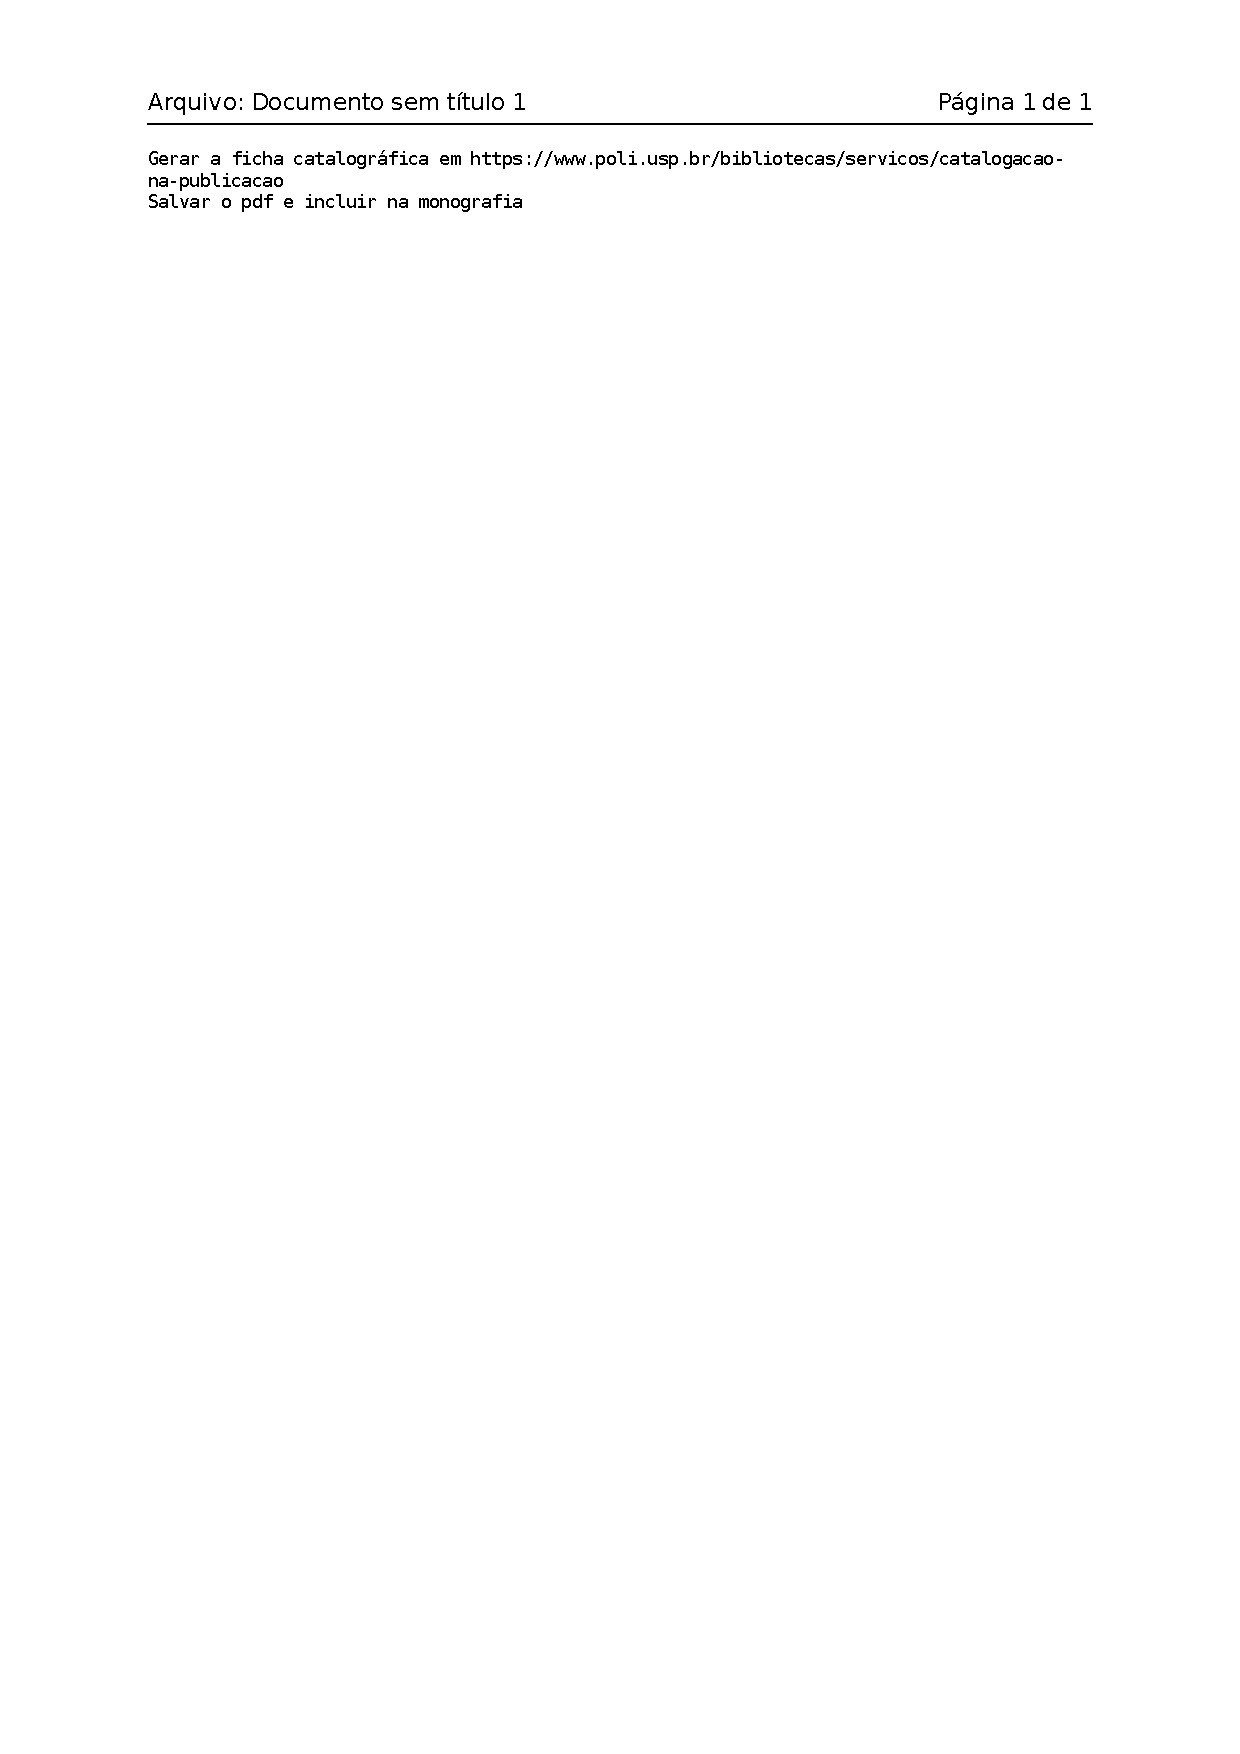
\includepdf{ficha.pdf}
% \end{fichacatalografica}

% \begin{fichacatalografica}
% 	\sffamily
% 	\vspace*{\fill}					% Posição vertical
% 	\begin{center}					% Minipage Centralizado
% 	\fbox{\begin{minipage}[c][8cm]{13.5cm}		% Largura
% 	\small
% 	\imprimirautor
% 	%Sobrenome, Nome do autor
	
% 	\hspace{0.5cm} \imprimirtitulo  / \imprimirautor. --
% 	\imprimirlocal, \imprimirdata-
	
% 	\hspace{0.5cm} \thelastpage p. : il. (algumas color.) ; 30 cm.\\
	
% 	\hspace{0.5cm} \imprimirorientadorRotulo~\imprimirorientador\\
	
% 	\hspace{0.5cm}
% 	\parbox[t]{\textwidth}{\imprimirtipotrabalho~--~\imprimirinstituicao,
% 	\imprimirdata.}\\
	
% 	\hspace{0.5cm}
% 		1. Palavra-chave1.
% 		2. Palavra-chave2.
% 		3. Palavra-chave3.
% 		I. Orientador.
% 		II. Universidade xxx.
% 		III. Faculdade de xxx.
% 		IV. Título 			
% 	\end{minipage}}
% 	\end{center}
% \end{fichacatalografica}
% ---

% ---
% Inserir errata
% ---
% \begin{errata}
% Elemento opcional da \citeonline[4.2.1.2]{NBR14724:2011}. Exemplo:

% \vspace{\onelineskip}

% FERRIGNO, C. R. A. \textbf{Tratamento de neoplasias ósseas apendiculares com
% reimplantação de enxerto ósseo autólogo autoclavado associado ao plasma
% rico em plaquetas}: estudo crítico na cirurgia de preservação de membro em
% cães. 2011. 128 f. Tese (Livre-Docência) - Faculdade de Medicina Veterinária e
% Zootecnia, Universidade de São Paulo, São Paulo, 2011.

% \begin{table}[htb]
% \center
% \footnotesize
% \begin{tabular}{|p{1.4cm}|p{1cm}|p{3cm}|p{3cm}|}
%   \hline
%    \textbf{Folha} & \textbf{Linha}  & \textbf{Onde se lê}  & \textbf{Leia-se}  \\
%     \hline
%     1 & 10 & auto-conclavo & autoconclavo\\
%    \hline
% \end{tabular}
% \end{table}

% \end{errata}
% ---

% ---
% Inserir folha de aprovação
% ---

% Isto é um exemplo de Folha de aprovação, elemento obrigatório da NBR
% 14724/2011 (seção 4.2.1.3). Você pode utilizar este modelo até a aprovação
% do trabalho. Após isso, substitua todo o conteúdo deste arquivo por uma
% imagem da página assinada pela banca com o comando abaixo:
%
% \begin{folhadeaprovacao}
% \includepdf{folhadeaprovacao_final.pdf}
% \end{folhadeaprovacao}
%
% \begin{folhadeaprovacao}

%   \begin{center}
%     {\ABNTEXchapterfont\large\imprimirautor}

%     \vspace*{\fill}\vspace*{\fill}
%     \begin{center}
%       \ABNTEXchapterfont\bfseries\Large\imprimirtitulo
%     \end{center}
%     \vspace*{\fill}
    
%     \hspace{.45\textwidth}
%     \begin{minipage}{.5\textwidth}
%         \imprimirpreambulo
%     \end{minipage}%
%     \vspace*{\fill}
%    \end{center}
        
%    Trabalho aprovado. \imprimirlocal, 24 de novembro de 2012:

%    \assinatura{\textbf{\imprimirorientador} \\ Orientador} 
%    \assinatura{\textbf{Professor} \\ Convidado 1}
%    \assinatura{\textbf{Professor} \\ Convidado 2}
%    %\assinatura{\textbf{Professor} \\ Convidado 3}
%    %\assinatura{\textbf{Professor} \\ Convidado 4}
      
%    \begin{center}
%     \vspace*{0.5cm}
%     {\large\imprimirlocal}
%     \par
%     {\large\imprimirdata}
%     \vspace*{1cm}
%   \end{center}
  
% \end{folhadeaprovacao}
% ---

% ---
% Dedicatória
% ---
% \begin{dedicatoria}
%    \vspace*{\fill}
%    \centering
%    \noindent
%    \textit{Finjo que não percebo, mas tudo está sendo observado. O esperto se faz de bobo para ver até onde o burro se faz de inteligente. Neste jogo sutil, cada movimento é estratégico e cada palavra esconde um significado oculto.} \vspace*{\fill}
% \end{dedicatoria}
% ---

% ---
% Agradecimentos
% ---
% \begin{agradecimentos}
% Agradecemos à todos os colegas e professores que tornaram possível e proveito o caminho até aqui.

% \end{agradecimentos}
% ---

% ---
% Epígrafe
% ---
% \begin{epigrafe}
%     \vspace*{\fill}
% 	\begin{flushright}
% 		\textit{...}
% 	\end{flushright}
% \end{epigrafe}
% ---

% ---
% RESUMOS
% ---

% resumo em português
\setlength{\absparsep}{18pt} % ajusta o espaçamento dos parágrafos do resumo
\begin{resumo}
O sistema On-Board Diagnostics II (OBD-II) é amplamente utilizado em veículos modernos para monitoramento e diagnóstico. Muitos dongles OBD-II comerciais que transmitem dados remotamente via Bluetooth ou Wi-Fi para aplicativos móveis apresentam vulnerabilidades documentadas, como ausência de autenticação, falta de criptografia e possibilidade de injeção de comandos no barramento CAN. Este trabalho propõe o desenvolvimento de um dongle e um companion app seguros, baseados no ESP32, incorporando autenticação mútua, criptografia, filtragem de mensagens CAN e proteção de firmware. A solução será validada contra as vulnerabilidades catalogadas e disponibilizada como projeto open source.

 \textbf{Palavras-chave}: : OBD-II. Segurança automotiva. Barramento CAN. Criptografia. ESP32. IoT veicular.
\end{resumo}

% resumo em inglês
\begin{resumo}[Abstract]
 \begin{otherlanguage*}{english}
   The On-Board Diagnostics II (OBD-II) system is widely used in modern vehicles for monitoring and diagnostic. Many comercial OBD-II dongles that wirelessly transmit data to companion apps via Bluetooth or Wi-Fi present documented vulnerabilities, including absent authentication, unencrypted communications, and arbitrary CAN command injection. This work proposes the development of a secure dongle and companion app based on the ESP32, incorporating mutual authentication, cryptography, CAN message filtering, and firmware integrity verification. The solution will be validated against the catalogued vulnerbilities and released as an open source project.

   \vspace{\onelineskip}
 
   \noindent 
   \textbf{Keywords}: OBD-II. Automotive security. CAN bus. 
   Cryptography. ESP32. Vehicular IoT.
 \end{otherlanguage*}
\end{resumo}

% % resumo em francês 
% \begin{resumo}[Résumé]
%  \begin{otherlanguage*}{french}
%     Il s'agit d'un résumé en français.
 
%    \textbf{Mots-clés}: latex. abntex. publication de textes.
%  \end{otherlanguage*}
% \end{resumo}

% % resumo em espanhol
% \begin{resumo}[Resumen]
%  \begin{otherlanguage*}{spanish}
%    Este es el resumen en español.
  
%    \textbf{Palabras clave}: latex. abntex. publicación de textos.
%  \end{otherlanguage*}
% \end{resumo}
% ---

% ---
% inserir lista de ilustrações
% ---
\pdfbookmark[0]{\listfigurename}{lof}
\listoffigures*
\cleardoublepage
% ---

% ---
% inserir lista de quadros
% ---
% \pdfbookmark[0]{\listofquadrosname}{loq}
% \listofquadros*
% \cleardoublepage
% ---

% ---
% inserir lista de tabelas
% ---
\pdfbookmark[0]{\listtablename}{lot}
\listoftables*
\cleardoublepage
% ---

% ---
% inserir lista de abreviaturas e siglas
% ---
\begin{siglas}
  \item[\textbf{IoT}] Internet of Things
  \item[\textbf{OBD-II}] On-Board Diagnostic II
  \item[\textbf{CAN}] Controller Area Network
  \item[\textbf{ECU}] Electronic Control Unit
  \item[\textbf{DTC}] Diagnostic Trouble Code
  \item[\textbf{PID}] Parameter Identification
  \item[\textbf{BLE}] Bluetooth Low Energy
  \item[\textbf{BLE}] Free Real-Time Operating System
  \item[\textbf{DoS}] Denial of Service
  \item[\textbf{AES}] Advanced Encryption Standard
  \item[\textbf{GCM}] Galois/Counter Mode
  \item[\textbf{ECDH}] Elliptic Curve Diffie-Hellman
  \item[\textbf{PCB}] Printed Circuit Board
  \item[\textbf{RM-ODP}] Reference Model for Open Distributed Processing
  \item[\textbf{MVP}] Minimal Viable Product
\end{siglas}
% ---

% ---
% inserir lista de símbolos
% ---
% \begin{simbolos}
%   \item[$ \Gamma $] Letra grega Gama
%   \item[$ \Lambda $] Lambda
%   \item[$ \zeta $] Letra grega minúscula zeta
%   \item[$ \in $] Pertence
% \end{simbolos}
% ---

% ---
% inserir o sumario
% ---
\pdfbookmark[0]{\contentsname}{toc}
\tableofcontents*
\cleardoublepage
% ---


% ----------------------------------------------------------
% ELEMENTOS TEXTUAIS
% ----------------------------------------------------------
\textual

% Capítulo 1. Introdução

\chapter{Introdução} \label{cap:intro}

Veículos modernos são compostos por uma variedade de sistemas eletrônicos responsáveis pelo monitoramento e pelo controle de diversos subsistemas do automóvel \cite{sonko2024embedded}. Nesse contexto, destaca-se o sistema On-Board Diagnostics II (OBD-II), um padrão de diagnóstico embarcado que permite o monitoramento de parâmetros do veículo e a identificação de falhas nos seus componentes eletrônicos e mecânicos \cite{csselectronics_obd2_intro}. 

O OBD-II foi inicialmente desenvolvido com o objetivo de facilitar a detecção de falhas relacionadas às emissões de poluentes, permitindo um diagnóstico mais rápido e preciso \cite{sonko2024embedded}.  Ao longo do tempo, tornou-se um componente essencial na arquitetura de veículos modernos, sendo utilizado para monitoramento de sensores e leitura de códigos de erros \cite{csselectronics_obd2_intro}. No Brasil, a adoção deste sistema tornou-se obrigatória para todos os veículos leves a combustão produzidos ou importados a partir de 2011 por meio da Resolução CONAMA nº 354/2004 \cite{conama354_2004}, o que evidencia sua prevalência e sua importância.

Com a popularização do OBD-II, surgiram dispositivos conhecidos como \textit{dongles} OBD-II, que se conectam à porta de diagnóstico do veículo. Esses sistemas podem coletar dados do veículo em tempo real e transmiti-los para outros sistemas, normalmente através de comunicações sem fio como o Bluetooth ou o Wi-fi \cite{wen2020plugnpwned}. Frequentemente, estes \textit{dongles} são utilizados em conjunto com aplicativos móveis, conhecidos como \textit{companion apps}, que permitem analisar, visualizar e processar os dados coletados, ou até mesmo enviar mensagens ao barramento CAN \cite{companionapps2024security}.

Esta combinação de \textit{dongles} e \textit{companion apps} abriu espaço para o desenvolvimento de diversas aplicações no contexto automotivo. Com a coleta de dados através de \textit{dongles} conectados à porta OBD-II, constróem-se sistemas de gerenciamento de frotas, estabelecendo-se um monitoramento operacional e logístico  \cite{malekian2017fleet}; sistemas de identificação de motorista, que classificam os motoristas em perfis de condução baseados em sua “agressividade” \cite{barreto2018perfis}, o que por sua vez abre espaço para a oferta de seguros com prêmio personalizado \cite{michailidis2025mlobd}; e técnicas de manutenção preventiva  \cite{errezgouny2025predictive}.

A maioria destas aplicações pressupõe que o \textit{dongle} permaneça conectado ininterruptamente à porta OBD-II, de modo a coletar os dados continuamente. Esta necessidade contrasta com evidências de que diversos \textit{dongles} OBD-II disponíveis comercialmente apresentam vulnerabilidades de segurança \cite{wen2020plugnpwned}. Além disso, os próprios \textit{companion apps} associados a esses dispositivos também apresentam vulnerabilidades, possibilitando a realização de ataques mesmo por indivíduos que não possuam conhecimento aprofundado sobre o funcionamento interno dos sistemas envolvidos \cite{companionapps2024security}.

%%%%%%%%%%%%%%%%%%%%%%%%%%
\section{Objetivos}

O presente trabalho propõe o projeto e a implementação de um \textit{dongle} OBD-II e de
um \textit{companion app} com foco em segurança. O objetivo é desenvolver uma solução
que mantenha a funcionalidade esperada (leitura de parâmetros e DTCs) ao mesmo
tempo em que incorpore mecanismos robustos de autenticação, criptografia, proteção de
firmware e controle de acesso ao barramento CAN, mitigando as vulnerabilidades
catalogadas pelo \textit{Donglescope} \cite{wen2020plugnpwned}, e habilitando a utilização segura
do OBD-II para diferentes aplicações, como gerenciamento de frotas \cite{malekian2017fleet}, identificação do perfil do motorista \cite{barreto2018perfis}, personalização de seguro \cite{michailidis2025mlobd}, e técnicas de manutenção preventiva  \cite{errezgouny2025predictive}.

Almeja-se um protótipo funcional de um \textit{dongle} OBD-II e de um \textit{companion app} projetados com foco em segurança. A solução deverá ser capaz de realizar a leitura de parâmetros padronizados do veículo obtidos por meio da interface OBD-II, tais como códigos de erro (DTCs) gerados pelo sistema de autodiagnóstico do carro e dados de sensores e variáveis operacionais do motor, incluindo rotação do motor, velocidade do veículo, temperatura do líquido de arrefecimento e posição do acelerador. Esses dados serão acessados por meio de \textit{Parameter IDs} (PIDs) definidos pelo padrão OBD-II. 

Do ponto de vista de segurança, espera-se que a solução proposta incorpore mecanismos capazes de mitigar as vulnerabilidades identificadas em dispositivos comerciais. Entre os resultados esperados estão a implementação de autenticação entre o \textit{dongle} e o aplicativo móvel, proteção criptográfica da comunicação sem fio e controle de acesso às mensagens enviadas ao barramento CAN. Para isso, pretende-se avaliar o sistema por meio de testes de segurança inspirados nos métodos utilizados em trabalhos da literatura, verificando se as principais vulnerabilidades descritas são mitigadas pela arquitetura proposta.

Por fim, espera-se que este trabalho contribua para o avanço da segurança em dispositivos automotivos conectados, fornecendo uma referência de arquitetura e de boas práticas para o desenvolvimento de \textit{dongles} OBD-II e aplicações associadas com maior nível de proteção contra ataques.


\section{Organização do Trabalho}

A \autoref{cap:intro} explica como o OBD-II possibilita a coleta de dados do automóvel em tempo real, que por sua vez ensejam uma miríade de aplicações. Explicitam-se os objetivos de projeto e desenvolvimento de um \textit{dongle} e de um \textit{companion app} seguros.

\autoref{cap:conceitos} apresenta elementos conceituais relacionados ao trabalho, e analisa as principais referências da literatura utilizadas e também os conceitos de engenharia mais importantes aplicados no projeto. Preocupa-se também com a modelagem dos ataques.

No \autoref{cap:especificacao}, de especificação, são descritos de maneira técnicas e completa todos os requisitos funcionais e não funcionais que foram planejados para o \textit{dongle}  e para o \textit{companion app}  que serão desenvolvidos no trabalho.  Nele, também é introduzida a arquitetura do sistema.

Com a especificação do projeto melhor definida, o \autoref{cap:desenvolvimento} foca na sua execução prática, apresentando o cronograma detalhado de como o projeto será realizado dentro do tempo disponível para o trabalho.

Por fim, no \autoref{cap:consideracoes}, de considerações finais, o trabalho é encerrado, com destataque para as constribuições técnicas relevantes para o contexto da engenharia: reprodutibilidade, segurança \textit{open source} para estudos e melhorias dentro da comunidade de \textit{dongles} automotivos e contribuição acadêmica na implementação de um protocolo seguro para a interação com a rede do veículo.

% Capítulo 2. Aspectos Conceituais
\chapter{Aspectos Conceituais} \label{cap:conceitos}

Para realizar a ambição de desenvolver um \textit{dongle} seguro, é necessário entender, primeiramente, o contexto no qual este dispositivo atuará; as especificações às quais ele deve sujeitar-se; e as possibilidades que fornecerá ao seu usuário.

A coleta dos dados é possibilitada pela existência da rede CAN, uma rede veicular que toma a forma de um barramento de dois fios, pelos quais trafegam as mensagens trocadas entre as ECUs. Ela será devidamente detalhada na seção \autoref{sec:CAN}; presentemente basta identificar que a rede CAN define somente as camadas física e de dados. Um protocolo de alto nível é necessário para gerenciar a comunicação e padronizar as mensagens.

Neste contexto, o protocolo OBD-II é adotado. Ele especifica, entre outros, a forma da comunicação, que ocorre no modelo requisição-resposta, e o formato das mensagens e dos dados nelas contidos. Também será oportunamente detalhado na \autoref{sec:OBD}. 

Nota-se que um dispositivo que deseje participar de comunicação OBD-II com um automóvel deve conectar-se à rede CAN do carro e saber modular suas mensagens nos dois fios que compõem o barramento, bem como identificar neles a resposta à sua requisição. Este é um processo trabalhoso e convidativo à abstração. Isto levou ao surgimento do ELM327, um \textit{dongle} que se conecta à porta OBD-II e fornece uma interface serial para um cliente, comumente um PC, que pode enviar e receber mensagens ASCII, as quais serão traduzidas para o formato das mensagens OBD-II. 

A implementação do \textit{dongle} proposto tomará, como modelo, o ELM327, cuja inspiração materializar-se-á em uma camada responsável por receber e enviar caracteres, processar comandos AT de autoconfiguração, e filtrar mensagens. Os pontos relevantes do ELM327 serão detalhados na seção \autoref{sec:ELM}.

O ESP32 é um microcontrolador (...) e será utilizado para implementação do \textit{dongle} proposto. Para possibilitar a integração do \textit{dongle} com um aplicativo móvel, optou-se pela utilização do Bluetooth Low Energy. Para a programação do ESP32, optou-se pela utilização do PlatformIO e freetros  

O microcontrolador escolhido para a implementação do \textit{dongle} proposto 
é o ESP32, um sistema em chip (SoC) que integra, entre outros periféricos, 
um controlador CAN e um módulo de comunicação Bluetooth, tornando-o adequado 
para os requisitos do projeto. Para possibilitar a integração do 
\textit{dongle} com um aplicativo móvel, optou-se pela utilização do 
Bluetooth Low Energy. Já para a programação do ESP32, optou-se pela 
utilização do FreeRTOS, um sistema operacional de tempo real que permitirá 
a organização do firmware em tarefas concorrentes, e do PlatformIO, ambiente 
de desenvolvimento que facilita o gerenciamento de dependências e a 
compilação do projeto.

// ADICIONAR PEQUENO PARAGRAFO SOBRE DART E APP

Com isso, estão dispostas todas as camadas que compõem o cenário do projeto, e cujo entendimento será indispensável para sua implementação. As seções seguintes, portanto, dedicar-se-ão ao detalhamento de cada uma delas.

\begin{figure}[H]
    \centering
    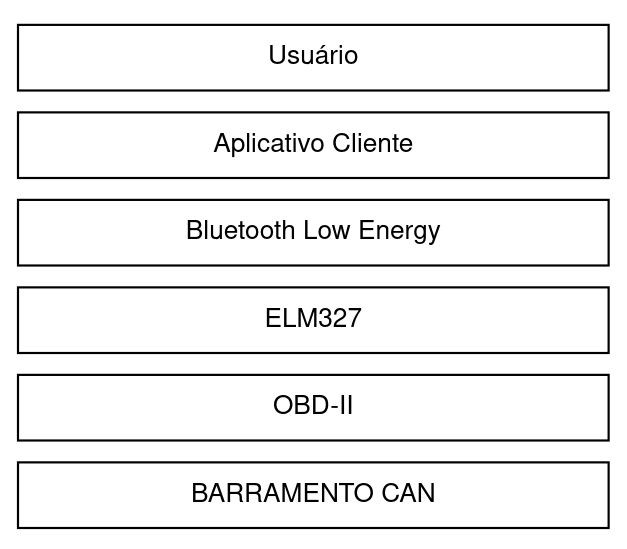
\includegraphics[width=0.6\textwidth]{assets/cap2-conceitos/camadas.png}
    \caption{Camadas que compõem o cenário do projeto}
    \label{fig:camadas}
    \fonte{Os autores (2026)}
\end{figure}


\section{Rede CAN} \label{sec:CAN}

A rede CAN foi especificada pela Bosch na década de 80 (TODO: MELHORAR), e é utilizada em veículos para permitir a comunicação confiável entre as suas unidades controladoras eletrônicas (ECUs). Ela especifica a camada física e a camada de dados.

DIAGRAMA DO BARRAMENTO CAN

EXPLICAÇÃO PREOCUPAÇÕES CAN - RELIABILITY; DETECÇÃO DE ERRO; DETECÇÃO DE COLLISÃO; ARBITRAGEM NÃO DESTRUTIVA 

EXPLICAÇÃO CONTROLADOR CAN - ADESÃO AO  PROTOCOLO CAN; ENCODING; ERROR DETECTION; ARBITRAGEM; SELF-DISCONNECT AO IDENTIFICAR MAU FUNCIONAMENTO PARA EVITAR ATRAPALHAR O BARRAMENTO; ETC

EXPLICAÇÃO TRANSCEIVER CAN - CONVERTE SINAIS LÓGICOS ÀS TENSÕES FÍSICAS NAS DUAS LINHAS DO BARRAMENTO

EXPLICAÇÃO FORMATOS DE UMA MENSAGEM CAN; DESTAQUE AO CAMPO "DATA", QUE CONTERÁ AS MENSAGENS OBD-II

\section{Protocolo OBD-II} \label{sec:OBD}

OBD-II REQUER QUE A CAMADA FÍSICA SUBJACENTE SEJA CAN; PODE SER 250 Kbits OU 500 kbits; O CAMPO CAN ID PODE TER 11 bits OU 29 bits; CAN IDS ESPECÍFICOS SÃO UTILIZADOS PARA REQUISIÇÕES E RESPOSTAS OBD; AS RESPOSTAS PODEM CABER EM UMA ÚNICA MENSAGEM (SINGLE FRAME) OU SERÃO DIVIDIDAS EM MÚLTIPLAS (MULTI-FRAME; ISO TP) 

OBD-II DEFINE CONECTOR; PINOS; EXPLICITAR QUE UM DOS PINOS É 12V, QUE É DA BATERIA DO CARRO

DIAGRAMA DOS CAMPOS DE UMA MENSAGEM OBD-II

EXPLICAÇÃO OBD-2 DEFINE SERVIÇOS (MODOS) E PIDS; EXPLICAÇÃO DOS PIDS PADRONIZADOS; PIDS DE DISCOVERY; ETC

TABELA COM PIDS PADRONIZADOS 

EXEMPLO DE UM CICLO REQUISIÇÃO-RESPOSTA OBD-II

EXPLICAÇÃO QUE UMA REQ PODE SER ATENDIDA POR MAIS DE UMA ECU

DIAGRAMA DE EXEMPLO DE UMA COMUNICAÇÃO ATENDIDA POR MAIS DE UMA ECU, COM FIRST FRAME, FLOW CONTROL, CONSECUTIVE FRAME

RESUMO DO QUE PODE SER CONSULTADO VIA OBD-II

\section{ELM327} \label{sec:ELM}

EXPLICAR QUE ELM-327 ORIGINALMENTE POSSIBILITA ASCII, MAS EXPLICITAR QUE SUA PREOCUPAÇÃO RESTRINGE-SE SOMENTE À TRADUÇÃO, CONFORME DOC:

""One must keep in mind that the ELM327 is a protocol interpreter that makes no attempt to assess the OBD messages for validity – it only ensures that hexadecimal digits were received, combined into bytes, then sent out the OBD port, and it does not know if a message sent to the vehicle was in error.""

EXPLICAR QUE PODE RECEBER COMANDOS AT PARA CONFIGURAÇÃO PRÓPRIA; EXEMPLOS DE COMANDOS AT. 

EXEMPLO DE COMUNICAÇÃO: ENVIA UM PID EM ASCII (EX. 010C ), RECEBE DADOS HEXADECIMAIS NA SAÍDA; CONVERTE ELES

COM ISTO DEVERÁ FICAR CLARO A COMUNICAÇÃO PONTA-A-PONTA.


\section{Bluetooth Low-Energy} \label{sec:BLE}

EXPLICAR O QUE É BLUETOOTH LOW ENERGY; DIFERENÇA AO CONVENCIONAL; GATT, SERVER, CLIENT, SERVICES, CHARACTERISTICS, GAP. SERIAL-OVER-BLE. NORDIC UUIDS PARA RX E TX.


\section{FreeRTOS e Arduino}

PARA QUE SERVE O FREERTOS; CONCEITOS BÁSICOS; TASKS; FILAS. 

\section{PlatformIO}

PLATFORMIO; VARIÁVEIS DE AMBIENTE; PERFIS DE COMPILAÇÃO

\section{Ataques}

MODELAGEM DE ATAQUES POSSÍVEIS

% Capítulo 3. Metodologia do Trabalho
\chapter{Método do trabalho} \label{cap:metodo}

%\begin{itemize}
%    \item Apresentar o processo de desenvolvimento do trabalho, através das suas fases (por exemplo, especificação de requisitos, projeto, implementação, testes). As fases dependem do tipo do trabalho e devem ser definidas com o apoio do orientador.
%    \item O desenvolvimento das fases e seus resultados devem estar descritos nos capítulos seguintes e não no capítulo de Método do Trabalho.
%    \item Citar os trabalhos consultados no texto.
%\end{itemize}

A metodologia adotada neste trabalho consiste no projeto, desenvolvimento e avaliação de um \textit{dongle} OBD-II seguro e de um \textit{companion app} capaz de interagir com ele de maneira confiável. O processo será dividido em quatro etapas principais: revisão bibliográfica e levantamento de requisitos, projeto da arquitetura do sistema, implementação da solução e avaliação de segurança.

Inicialmente será realizada uma revisão da literatura sobre o funcionamento do padrão OBD-II, do barramento CAN e das principais vulnerabilidades identificadas em \textit{dongles} comerciais. Essa etapa permitirá compreender as superfícies de ataque presentes nesses dispositivos e estabelecer os requisitos de segurança que deverão ser considerados no desenvolvimento da solução proposta.

Em seguida será realizado o projeto da arquitetura do sistema. A solução será composta por dois componentes principais: um \textit{dongle} conectado à porta OBD-II do veículo e um \textit{companion app} executado em um dispositivo móvel. O \textit{dongle} será responsável pela comunicação com o barramento CAN do veículo e pela coleta de dados diagnósticos, enquanto o aplicativo móvel será responsável pela visualização e pelo processamento dessas informações. A comunicação entre ambos será realizada por meio de um protocolo sem fio, como Bluetooth ou Wi-Fi.

Durante o projeto da arquitetura serão definidos mecanismos de segurança voltados à mitigação das vulnerabilidades identificadas na literatura. Entre esses mecanismos destacam-se: autenticação entre o \textit{dongle} e o aplicativo móvel, utilização de criptografia para proteção da comunicação e implementação de mecanismos de controle de acesso às mensagens transmitidas ao barramento CAN.

Na etapa de implementação será desenvolvido um protótipo funcional do \textit{dongle}, baseado em um microcontrolador com suporte à comunicação CAN e a interfaces sem fio. Paralelamente será desenvolvido um \textit{companion app} capaz de estabelecer comunicação segura com o dispositivo, realizar a leitura de parâmetros do veículo e apresentar as informações ao usuário.

Por fim, será realizada uma etapa de avaliação de segurança da solução desenvolvida. Nessa fase serão conduzidos testes com o objetivo de verificar se o sistema é capaz de mitigar as vulnerabilidades discutidas na literatura. Para isso serão utilizados testes inspirados nos procedimentos descritos em estudos anteriores, buscando verificar aspectos como autenticação, controle de acesso à comunicação e proteção contra injeção de comandos CAN não autorizados.



% Capítulo 4. Especificação de Requisitos
\chapter{Especificação do Sistema} \label{cap:especificacao}

A fim de realizar uma especificação do projeto completa e adequada frente ao contexto abordado e aos objetivos desejados, é proveitoso adotar um referencial teórico formal para orientar esse processo metodologicamente. Nesse sentido, o modelo adotado foi uma versão adaptada do \textit{Reference Model for Open Distributed Processing} (RM-ODP) \cite{tcc-rmodp}, o qual preconiza o estabelecimento de diferentes visões sobre o sistema de modo a separar as responsabilidades e melhor guiar o desenvolvimento. Além disso, essa alternativa se vale de um arcabouço teórico bastante conhecido e robusto e se aplica de forma conveniente para a modelagem do tipo de sistema e aplicação do projeto, o que a torna uma escolha propícia para o trabalho.

Mais especificamente, são propostas quatro visões:

\begin{itemize}
    \item \textbf{Visão Empresarial:} Contextualiza o sistema, o problema que pretende abordar, seus objetivos, atores/stakeholders e motivações para a aplicação.
    \item \textbf{Visão de Requisitos:} Elenca e detalha apropriadamente todos os requisitos do sistema (incluindo e diferenciando entre funcionais e não funcionais) e é alicerçada na Visão Empresarial.
    \item \textbf{Visão de Arquitetura:} Determina a estrutura do sistema, abarcando desde componentes individuais até grandes módulos e a forma como se conectam. Seu propósito é possibilitar e favorecer o atendimento da Visão de Requisitos.
    \item \textbf{Visão Tecnológica:} Delimita a implementação concreta do sistema, desde frameworks de software a serem empregados até quais componentes físicos serão utilizados. Sua meta é permitir que a Visão de Arquitetura seja posta em prática e efetivada cumprindo os requisitos impostos.
\end{itemize}

No projeto, essas visões ajudam a guiar a especificação e já se mostram presentes, visto que a Empresarial foi elaborada nos capítulos anteriores e as demais são discorridas no presente capítulo. Dito isso, vale ressaltar que esse modelo ainda será revisitado continuamente ao longo da execução do trabalho, permitindo aprimorar e aprofundar alguns tópicos e realizar eventuais modificações que venham a ser necessárias.

% ===================================================================
\section{Requisitos Funcionais}
% ===================================================================
 
Os requisitos funcionais descrevem as capacidades que o sistema, composto pelo
\textit{dongle} OBD-II e pelo \textit{companion app}, deve oferecer. Cada requisito recebe um identificador único (\texttt{RF-XX}), uma descrição objetiva e uma
prioridade (\palta, \pmedia{} ou \pbaixa).
 
\subsection{Dongle OBD-II}
 
\begin{longtable}{p{1.5cm} p{11cm} p{2cm}}
\caption{Requisitos Funcionais do Dongle OBD-II}
\label{tab:rf-dongle-cap-especificacao} \\
\toprule
\textbf{ID} & \textbf{Descrição} & \textbf{Prioridade} \\
\midrule
\endfirsthead

\toprule
\textbf{ID} & \textbf{Descrição} & \textbf{Prioridade} \\
\midrule
\endhead
 
RF-01 &
Ler parâmetros do veículo via protocolo OBD-II (PIDs padrão: rotação do motor,
velocidade, temperatura do líquido de arrefecimento e posição do acelerador). &
\palta \\ \hline
 
RF-02 &
Ler e retornar Diagnostic Trouble Codes (DTCs) armazenados na ECU do veículo. &
\palta \\ \hline
 
RF-03 &
Estabelecer comunicação sem fio (BLE ou Wi-Fi) com o \textit{companion app},
transmitindo os dados coletados em tempo real. &
\palta \\ \hline
 
RF-04 &
Exigir autenticação mútua com o \textit{companion app} antes de executar as funcionalidades de coleta e transmissão de dados. &
\palta \\ \hline
 
RF-05 &
Cifrar todo o tráfego transmitido sem fio entre o \textit{dongle} e o
\textit{companion app}. &
\palta \\ \hline
 
RF-06 &
Filtrar mensagens CAN enviadas ao barramento, permitindo somente mensagens
diagnósticas pré-definidas e rejeitando qualquer comando arbitrário. &
\pmedia \\ \hline
 
RF-08 &
Suportar atualização de firmware (\textit{over-the-air}) somente mediante
verificação de assinatura criptográfica, rejeitando pacotes inválidos. &
\pbaixa \\ \hline
 
RF-09 &
Entrar em modo de pareamento (aceitar nova conexão) apenas mediante acionamento
de botão físico no dispositivo, por período limitado de tempo. & \pmedia \\ \hline
 
RF-10 &
Expor uma interface de diagnóstico que permita consultar o estado de saúde interno
do \textit{dongle} (versão de firmware, status de conexão, contadores de erro). &
\pbaixa \\
 
\bottomrule
\end{longtable}

A prioridade alta foi dada às tarefas que exigem uma conexção direta com o hardware e estabelecimento do protocolo de comunicação, uma vez que esses aspectos são imprescindíveis para qualquer estudo de segurança no contexto do trabalhoe representam também a maior barreira de aprendizem para o começo da prototipação.

As prioridades média e baixa foram dada a atividades que, apesar de não serem essenciais para o trabalho, seriam interessantes de serem implementados para uma cobertura completa das vulnerabilidades estudades. Dentre eles, o requisito RF-08 recebeu prioridade baixa por ser a implementação mais difícil, podendo não se encaixar no tempo do projeto; e o requisito RF-10 pelo fato de representar apenas uma ajuda visual, não impactando diretamente o funcionamento de um MVP do projeto.
 
\subsection{Companion App}
 
\begin{longtable}{p{1.5cm} p{11cm} p{2cm}}
\caption{Requisitos Funcionais do Companion App}
\label{tab:rf-app-cap-especificacao} \\
\toprule
\textbf{ID} & \textbf{Descrição} & \textbf{Prioridade} \\
\midrule
\endfirsthead

\toprule
\textbf{ID} & \textbf{Descrição} & \textbf{Prioridade} \\
\midrule
\endhead
 
RF-11 &
Descobrir, parear e conectar-se ao \textit{dongle} OBD-II de forma segura,
utilizando o protocolo de autenticação definido na arquitetura. &
\palta \\ \hline
 
RF-12 &
Exibir em tempo real os parâmetros lidos do veículo (PIDs) em telas de
visualização claras e navegáveis. &
\palta \\ \hline
 
RF-13 &
Apresentar e interpretar DTCs retornados pelo \textit{dongle}, informando ao
usuário o significado de cada código. &
\pmedia \\ \hline
 
RF-14 &
Exibir o histórico de leituras de odômetro recuperado do \textit{dongle},
alertando o usuário caso seja detectada inconsistência ou indício de adulteração. &
\pbaixa \\ \hline
 
RF-15 &
Conduzir o usuário pelo processo de pareamento via botão físico (RF-09),
orientando cada etapa por meio de instruções na interface. &
\pbaixa \\ \hline
 
RF-16 &
Permitir a exportação dos dados coletados em
formato aberto (CSV ou JSON) para uso externo. &
\pbaixa \\
 
\bottomrule
\end{longtable}

Na implementação do \textit{companion app}, foi dada prioridade alta para os elementos diretamente relacionados ao estudo de segurança, ou seja, pareamento e comunicação do \textit{dongle}.

O requisito RF-13 recebeu prioridade média pelo fato de, mesmo não sendo essencial para o trabalho a visualização de DTCs, a garantia de sua integridade é importante para garantir que nenhum atacante esteja influenciando na manutenção do veículo, ou seja, ainda representar um aspecto de segurança.

Os outros requisitos recebem prioridade baixa por não estarem relacionados com segurança.

 
% ===================================================================
\section{Requisitos Não Funcionais}
% ===================================================================
 
Os requisitos não funcionais estabelecem restrições de qualidade, desempenho,
segurança e conformidade que o sistema deve satisfazer. Cada requisito recebe um
identificador (\texttt{RNF-XX}) e uma prioridade.


\begin{longtable}{p{1.5cm} p{11cm} p{2cm}}
\caption{Requisitos Não-Funcionais do Sistema}
\label{tab:rnf-sistema-cap-especificacao} \\
\toprule
\textbf{ID} & \textbf{Descrição} & \textbf{Prioridade} \\
\midrule
\endfirsthead

\toprule
\textbf{ID} & \textbf{Descrição} & \textbf{Prioridade} \\
\midrule
\endhead

RNF-01 & 
Os dados transmitidos via interface sem fio devem ser protegidos por mecanismos de cifração que garantam a confidencialidade e integridade das informações. & 
\palta \\ \hline

RNF-02 & 
O sistema deve utilizar métodos de autenticação robustos para garantir que apenas dispositivos autorizados estabeleçam conexão com o hardware. & 
\palta \\ \hline

RNF-03 & 
O processo de atualização de firmware deve incluir mecanismos de verificação de origem e integridade para impedir a execução de código não autorizado. & 
\palta \\ \hline

RNF-04 & 
O sistema deve ser validado contra as principais vulnerabilidades de segurança documentadas na literatura para dispositivos de diagnóstico automotivo. & 
\palta \\ \hline

RNF-05 & 
O dispositivo deve operar em conformidade com as normas e padrões internacionais de diagnóstico veicular (ISO 15765-4 e SAE J1979). & 
\palta \\ \hline

RNF-06 & 
A latência de comunicação entre a coleta de dados no barramento e a visualização no aplicativo deve ser compatível com o monitoramento em tempo real. & 
\pmedia \\ \hline

RNF-07 & 
O sistema deve garantir a estabilidade da conexão sem fio e possuir mecanismos de recuperação automática em caso de desconexão momentânea. & 
\pmedia \\ \hline

RNF-08 & 
O software do aplicativo deve ser compatível com as versões atuais dos sistemas operacionais móveis predominantes no mercado. & 
\pmedia \\ \hline

RNF-09 & 
A arquitetura e o software elaborados, especialmente no que diz respeito ao dongle, devem ser compatíveis com dispositivo embarcado de baixo poder computacional. & 
\pmedia \\ \hline

RNF-10 & 
A arquitetura de software deve ser modular, seguindo boas práticas de desenvolvimento e padrões de projeto. & 
\pmedia \\ \hline

RNF-11 & 
A interface do usuário deve ser intuitiva, permitindo o acesso às funcionalidades principais com o mínimo de intervenção manual. & 
\pbaixa \\ 

\bottomrule
\end{longtable}

Nos requisitos não funcionais, recebem prioridade alta os requisitos relacionados a segurança, prioridade média os requisitos não relacionados a segurança que garantem a utilização do sistema seja confiável e compatível (RNF-06, RNF-07 e RNF-08), ou que estejam em linha com as contribuições do projeto (RNF-09 favorece reprodutibilidade e um projeto final mais econômico em termos financeiros e de uso de recursos, ao passo que RNF-10 também facilita reprodutibilidade e manutenção de base de código \textit{open source}).

\section{Arquitetura}


A arquitetura proposta para este trabalho foi concebida sob o princípio da modularidade. O sistema é segmentado em três domínios principais: a Camada Veicular, o Dongle OBD-II Seguro e o Companion App.

\subsection{Visão Geral e Fluxo de Dados}

O fluxo de informações inicia-se na Camada Veicular, onde os dados de diagnóstico são extraídos do barramento CAN através da porta física OBD-II \cite{csselectronics_obd2_intro}. O Dongle atua como uma ponte controlada, processando as requisições do usuário e aplicando políticas de filtragem \cite{wen2020plugnpwned}. Por fim, o Companion App funciona como a interface de controle e autenticação \cite{companionapps2024security}. A \autoref{fig:arquitetura-preliminar-cap-especificacao} exibe uma visão geral da arquitetura proposta.

\begin{figure}[H]
    \centering
    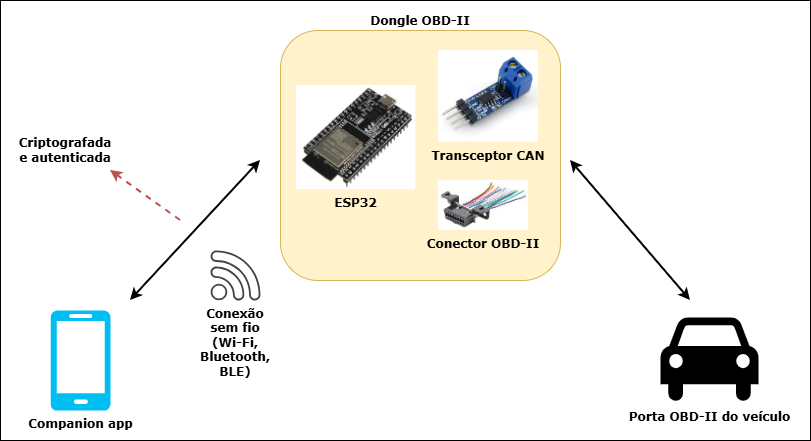
\includegraphics[width=0.9\linewidth]{assets/cap4-especificacao/arquitetura-preliminar.png}
    \caption{Arquitetura geral proposta para o sistema}
    \label{fig:arquitetura-preliminar-cap-especificacao}
\end{figure}

\subsection{Módulos do Dongle OBD-II}

O hardware é organizado em blocos lógicos, os quais incluem tanto componentes físicos quanto de software:

\begin{itemize}
    \item \textbf{Interface CAN:} Responsável pela sinalização física segundo o padrão ISO 15765-4 \cite{malekian2017fleet}.
    \item \textbf{Comunicação Sem Fio:} Permite que o sistema opere via Bluetooth ou Wi-Fi \cite{wen2020plugnpwned}.
    \item \textbf{Módulo de Segurança:} Centraliza as primitivas criptográficas para cifração e autenticação \cite{companionapps2024security}.
    \item \textbf{Filtro de Mensagens (Allow-list):} Atua como um \textit{firewall} para o barramento CAN, impedindo a injeção de comandos arbitrários \cite{wen2020plugnpwned}.
\end{itemize}

Do ponto de vista físico, o hardware tem como seu elemento central o microcontrolador ESP32, o qual consiste em um dispositivo acessível, com um poder computacional relativamente baixo (típico para aplicações embarcadas de borda) e que, ainda assim, conta com uma variedade de recursos oportunos, como módulos de comunicação sem fio (Wi-Fi e Bluetooth/BLE) e um controlador CAN embutido \cite{esp32-datasheet}. Assim, a placa fica responsável por efetivar a intermediação da comunicação entre o app e o veículo, implementando regras de negócio e mecanismos de segurança.

Para que um dispositivo possa se conectar a uma rede CAN, são necessários dois componentes especializados \cite{can_standard_overview}: um controlador CAN, responsável por implementar o protocolo lógico do enlace de dados, e um transceptor CAN, responsável por realizar as conversões de sinais para os formatos adequados de cada camada física. A \autoref{fig:can-conexao-cap-especificacao} ilustra esse esquema e suas interfaces.

\begin{figure}[H]
    \centering
    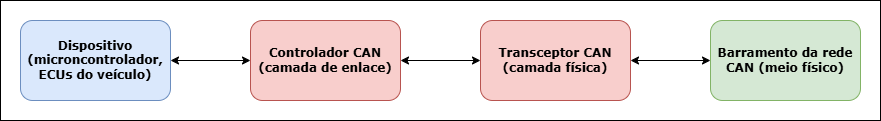
\includegraphics[width=0.9\linewidth]{assets/cap4-especificacao/conexao-can.png}
    \caption{Esquema geral de um nó de rede CAN}
    \label{fig:can-conexao-cap-especificacao}
\end{figure}

Desse modo, para possibilitar toda a comunicação do projeto, serão utilizados mais dois elementos: o transceptor CAN mencionado - a exemplo do SN65HVD230 \cite{SN65HVD23x-datasheet} - e um conector OBD-II para interfaceamento com a porta localizada no veículo, compondo assim o esquema da \autoref{fig:arquitetura-preliminar-cap-especificacao}.

\subsection{Arquitetura do Companion App}

O aplicativo móvel é estruturado para espelhar as garantias de segurança do hardware \cite{companionapps2024security}:

\begin{itemize}
    \item \textbf{Gerenciador de Conexão:} Responsável pela descoberta e link sem fio.
    \item \textbf{Núcleo de Cifração e Autenticação:} Utiliza armazenamento seguro como o Android Keystore \cite{companionapps2024security}.
    \item \textbf{Interpretador de Protocolo:} Realiza a tradução das respostas brutas do dongle.
\end{itemize}

\subsection{Modelo de Confiança e Comunicação Segura}

O sistema adota um modelo de segurança baseado na proximidade física para o pareamento inicial entre dongle e app \cite{wen2020plugnpwned}. A comunicação subsequente utiliza um esquema criptográfico para garantir a confidencialidade, integridade e autenticidade dos dados \cite{companionapps2024security}, o qual consiste essencialmente no uso inicial do ECDH como método assimétrico para obtenção de uma chave privada compartilhada e no uso do AES-GCM para cifração e autenticação simétricas das mensagens trocadas.


% Capítulo 5. Desenvolvimento do Trabalho
%\chapter{Desenvolvimento do Trabalho} \label{cap:desenvolvimento}

%\section{Tecnologias Utilizadas}
%Durante o desenvolvimento do trabalho, são utilizadas tecnologias e ferramentas adequadas. Essa seção deve apresentar as tecnologias e ferramentas mais relevantes, utilizadas no desenvolvimento. 

%\section{Projeto e Implementação}
%Descrever os resultados do projeto e da implementação do trabalho, com justificativas das decisões tomadas.

%\section{Testes e Avaliação}
%Descrever o procedimento da avaliação do trabalho (teste de hardware, teste de software, teste de módulo, teste de integração, teste de validação), de acordo com o tipo do sistema, com o apoio do orientador, se necessário.

\chapter{Desenvolvimento} \label{cap:desenvolvimento}
 % ===================================================================
\section{Cronograma}
% ===================================================================
 
O projeto é executado de abril a setembro de 2026, dividido em duas entregas
mensais. A \autoref{tab:cronograma-cap-desenvolvimento} e a \autoref{fig:diagrama-gantt-cap-desenvolvimento} apresentam o cronograma detalhado.
 
\begin{longtable}{p{1.8cm} p{6cm} p{6cm}}
\caption{Cronograma das atividades planejadas} \label{tab:cronograma-cap-desenvolvimento} \\
\toprule
\textbf{Mês} & \textbf{Entrega 1} & \textbf{Entrega 2} \\
\midrule
\endfirsthead

\toprule
\textbf{Mês} & \textbf{Entrega 1} & \textbf{Entrega 2} \\
\midrule
\endhead
 
\textbf{Abril} &
\textit{Setup} do projeto com FreeRTOS / ESP-IDF; implementação do \texttt{MockDataCollector}; estudos sobre a plataforma. &
Início da escrita do TCC: Introdução, Fundamentação Teórica (OBD-II, CAN, segurança) e Modelagem de Ameaças. \\ \hline
 
\textbf{Maio} &
Comunicação OBD-II via CAN (ESP32 + transceptor CAN conectado a simulador OBD-II); leitura de PIDs reais. &
Comunicação ESP32 $\leftrightarrow$ App, recebimento de dados em tempo real (via Wi-Fi ou BLE). \\ \hline
 
\textbf{Junho} &
Testes de segurança iniciais (\textit{Donglescope}); implementação do protocolo de autenticação mútua entre App e \textit{dongle}. &
Cifração do tráfego entre App e \textit{dongle} (AES-GCM + ECDH); integração com módulo de autenticação. \\ \hline
 
\textbf{Julho} &
Testes de segurança completos; redação dos capítulos de Arquitetura e Análise Comparativa com \textit{dongles} comerciais. &
Desenvolvimento das telas principais do App (visualização de PIDs, DTCs, odômetro). \\ \hline
 
\textbf{Agosto} &
\textit{Buffer} para absorção de atrasos e ajustes. &
\textit{Buffer} para absorção de atrasos e ajustes. \\ \hline
 
\textbf{Setembro} &
Consolidação da versão final do TCC; revisão geral do texto, correções e formatação. &
--- \\
 
\bottomrule
\end{longtable}

\begin{figure}[H]
    \centering
    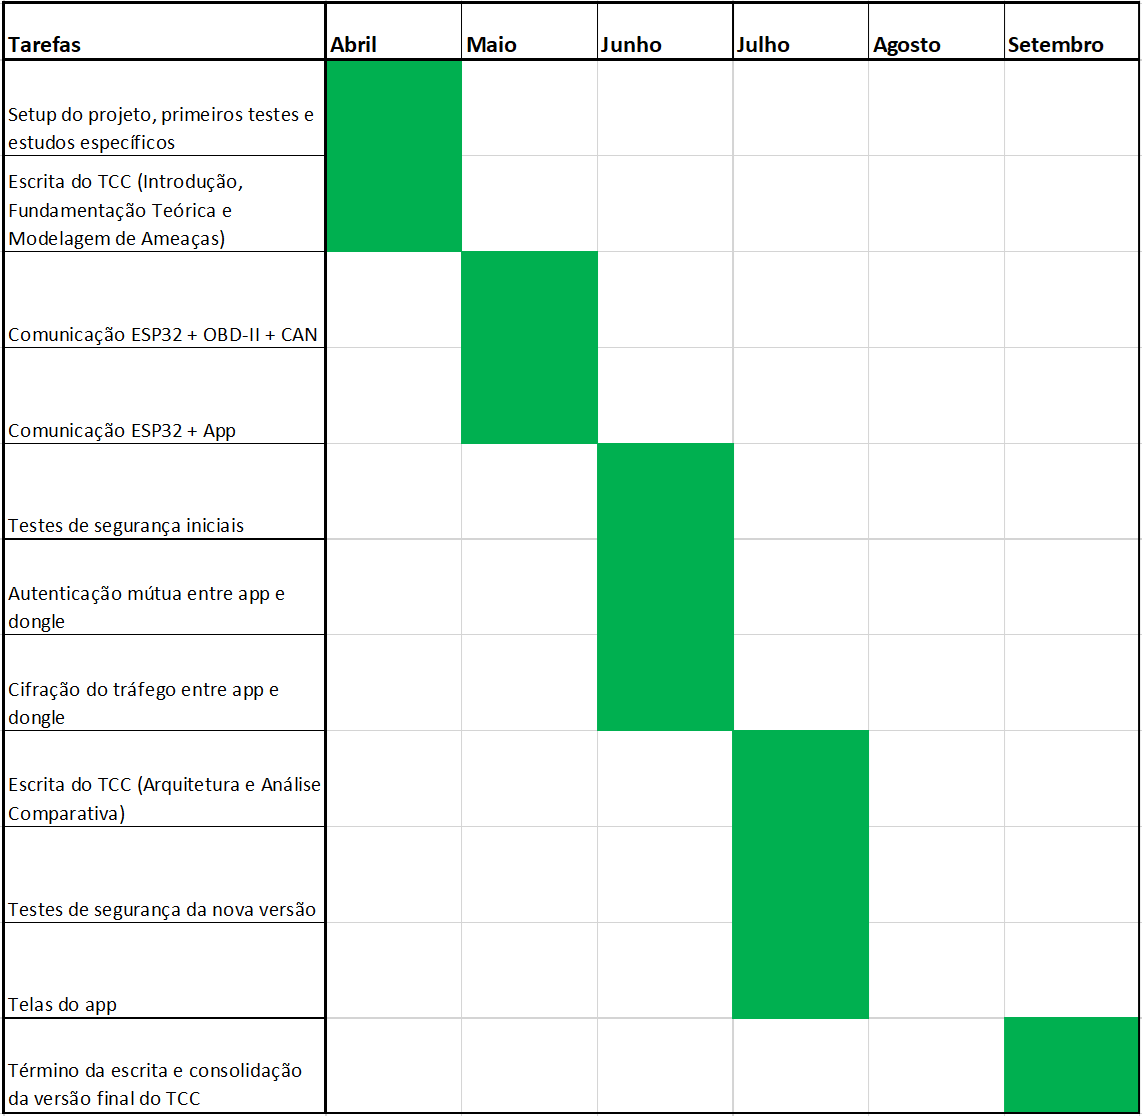
\includegraphics[width=0.9\linewidth]{assets/cap5-desenvolvimento/gantt.png}
    \caption{Diagrama de Gantt das atividades planejadas}
    \label{fig:diagrama-gantt-cap-desenvolvimento}
\end{figure}


% ---
% Capitulo com exemplos de comandos inseridos de arquivo externo 
% ---
% \include{abntex2-modelo-include-comandos}
% ---
% Conteúdos específicos do modelo de trabalho acadêmico
% \include{quadros}

% ----------------------------------------------------------
% Finaliza a parte no bookmark do PDF
% para que se inicie o bookmark na raiz
% e adiciona espaço de parte no Sumário
% ----------------------------------------------------------
\phantompart

% ---
% Conclusão
% ---
% Capítulo 6. Considerações Finais
\chapter{Considerações Finais} \label{cap:consideracoes}

%\section{Conclusões do Projeto de Formatura}
%Apresentar o balanço do trabalho: resultados atingidos e não atingidos, com justificativas.

\section{Contribuições}
Além dos resultados práticos do protótipo, este trabalho apresenta três contribuições
técnicas de caráter mais amplo à comunidade de Engenharia:
 
\subsection{Reprodutibilidade por meio do ESP32}
 
O \textit{dongle} é construído sobre o microcontrolador \textbf{ESP32}, um
componente amplamente disponível, de baixo custo e bem documentado. Essa escolha
garante que qualquer pesquisador, estudante ou profissional possa reproduzir,
adaptar ou estender o hardware sem dependência de componentes proprietários ou de
difícil aquisição. Todo o esquemático, \textit{layout} de PCB e código-fonte do
firmware serão disponibilizados publicamente, tornando o trabalho integralmente
reprodutível.
 
\subsection{Entregável \textit{Open Source} como Base para Pesquisas Futuras}
 
O \textit{dongle} desenvolvido será publicado como projeto \textit{open source}
(hardware e software), servindo como plataforma de referência para pesquisas que
demandem coleta de dados veiculares confiáveis. Trabalhos nas áreas de
\textit{driver behavior}, manutenção preditiva, controle de frotas e detecção de
anomalias em barramentos CAN poderão utilizar o entregável como ponto de partida,
sem precisar lidar com as vulnerabilidades presentes nos \textit{dongles} comerciais
atualmente disponíveis.
 
\subsection{Protocolo Padronizado e Seguro de Comunicação OBD-II}
 
A principal lacuna identificada na literatura é a ausência de um protocolo
padronizado de comunicação entre \textit{dongles} OBD-II e \textit{companion apps}
que incorpore requisitos de segurança desde a sua concepção. Este trabalho irá implementar um protocolo baseado no existente ELM-327 \cite{elm327datasheet}, porém com considerações de segurança que atendam os serviços de integridade, confidencialidade e autenticidade.

 
%\section{Perspectivas de Continuidade}
%Descrever os trabalhos que podem ser realizados como continuação do projeto de formatura.

% ----------------------------------------------------------
% ELEMENTOS PÓS-TEXTUAIS
% ----------------------------------------------------------
\postextual
% ----------------------------------------------------------

% ----------------------------------------------------------
% Referências bibliográficas
% ----------------------------------------------------------
\bibliography{abntex2-modelo-references}

% ----------------------------------------------------------
% Glossário
% ----------------------------------------------------------
%
% Consulte o manual da classe abntex2 para orientações sobre o glossário.
%
%\glossary

% ----------------------------------------------------------
% Apêndices
% ----------------------------------------------------------

% ---
% Inicia os apêndices
% ---
% \begin{apendicesenv}

% % Imprime uma página indicando o início dos apêndices
% \partapendices

% % ----------------------------------------------------------
% \chapter{Quisque libero justo}
% % ----------------------------------------------------------

% \lipsum[50]

% % ----------------------------------------------------------
% \chapter{Nullam elementum urna vel imperdiet sodales elit ipsum pharetra ligula
% ac pretium ante justo a nulla curabitur tristique arcu eu metus}
% % ----------------------------------------------------------
% \lipsum[55-57]

% \end{apendicesenv}
% % ---


% ----------------------------------------------------------
% Anexos
% ----------------------------------------------------------

% ---
% Inicia os anexos
% ---
% \begin{anexosenv}

% % Imprime uma página indicando o início dos anexos
% \partanexos

% % ---
% \chapter{Morbi ultrices rutrum lorem.}
% % ---
% \lipsum[30]

% % ---
% \chapter{Cras non urna sed feugiat cum sociis natoque penatibus et magnis dis
% parturient montes nascetur ridiculus mus}
% % ---

% \lipsum[31]

% % ---
% \chapter{Fusce facilisis lacinia dui}
% % ---

% \lipsum[32]

% \end{anexosenv}

%---------------------------------------------------------------------
% INDICE REMISSIVO
%---------------------------------------------------------------------
\phantompart
\printindex
%---------------------------------------------------------------------

\end{document}